\chapter{Graphs}

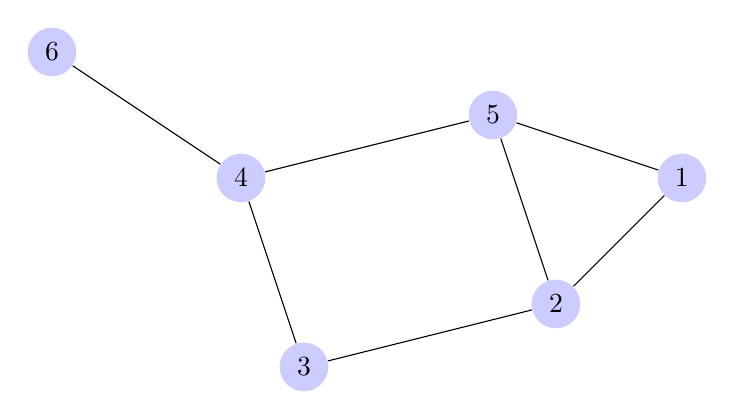
\begin{tikzpicture}
[scale=.8,auto=left,every node/.style={circle,fill=blue!20}]
\node (n6) at (1,10) {6};
\node (n4) at (4,8)  {4};
\node (n5) at (8,9)  {5};
\node (n1) at (11,8) {1};
\node (n2) at (9,6)  {2};
\node (n3) at (5,5)  {3};

\foreach \from/\to in {n6/n4,n4/n5,n5/n1,n1/n2,n2/n5,n2/n3,n3/n4}
\draw (\from) -- (\to);

\end{tikzpicture}












\begin{tikzpicture}
[scale=.8,auto=left,every node/.style={circle,fill=blue!20}]
\tikzset{vertex/.style = {shape=circle,draw,minimum size=1.5em}}
\tikzset{edge/.style = {->,> = latex'}}

  \node (s) at (0,5){source};
    \node (v1) at (5,9){alpha};
      \node (v4) at (13,9){beta};
        \node (v2) at (5,1){omega};
          \node (v3) at (6,5){gamma};
            \node (v5) at (13,1){theta};
              \node (v6) at (16,5){delta};
                \node (t) at (20,5){sink};

                \tikzset{EdgeStyle/.style={->}}
                \Edge[label=$1/1$](s)(v1);
                \Edge[label=$4/4$](s)(v2);
                \Edge[label=$2/2$](s)(v3);
                \Edge[label=$2/2$](v2)(v4);
                \Edge[label=$2/2$](v2)(v5);
                \Edge[label=$1/1$](v1)(v4);
                \Edge[label=$1/1$](v3)(v4);
                \Edge[label=$4/4$](v6)(t);
                \Edge[label=$1/1$](v5)(t);
                \Edge[label=$2/2$](v4)(t);
                \Edge[label=$1/4$](v5)(v6);
                \Edge[label=$1/1$](v3)(v6);
                \Edge[label=$2/2$](v4)(v6);

                \draw[dashed] 
                  ([yshift=60pt]$ (s)!0.5!(v1) $ ) -- 
                    ([yshift=-60pt]$ (s)!0.5!(v2) $ );

                    \end{tikzpicture}
